\section{Toolkit Overview}
In this section, we first introduce the design decisions and the overview of the toolkits. Then we present the user interface and the major functions.

Firstly, the toolkit is designed and implemented as a web application, since it is easiest for crowd workers to visit.

The users of our visualization toolkit include {\em annotation gatherers} and {\em crowd-source workers}. In general, annotation gatherers use our toolkit to collect training data from crowd-source workers for their NLP systems. It is reasonable to assume they are NLP experts and well-trained programmers. We believe annotation gatherers know their NLP problems better than anyone else, so we leave them to implement the visualization of the NLP task by implementing a static page. They should embed the APIs of our toolkits in their html so they can pass on the objects to cluster or parse. We keep the task-visualization transparent to maximize the flexibility of our toolkit. Figure~\ref{fig:workflow} shows the workflow of our toolkit.

\begin{figure}
\centering
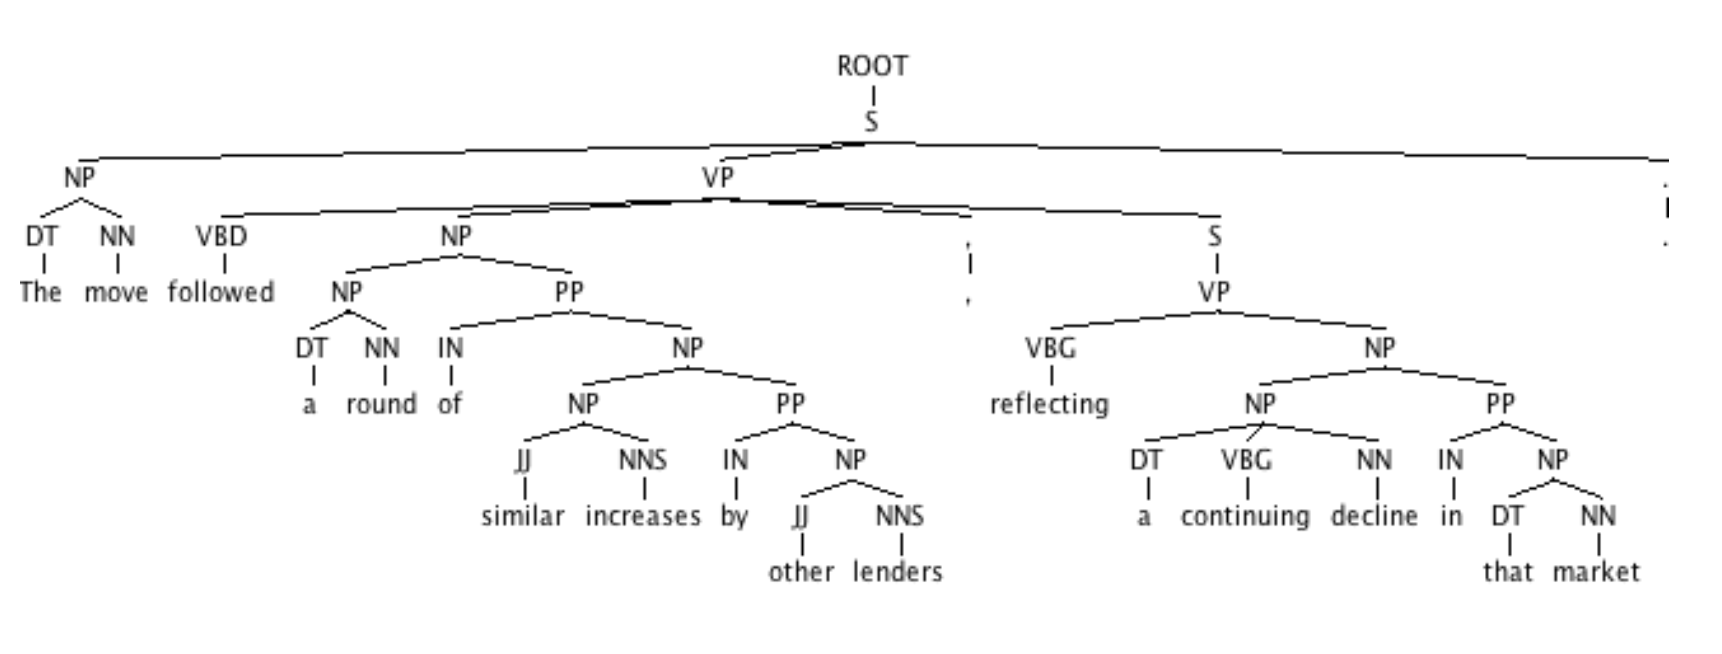
\includegraphics[width=3.1in]{figs/parsetree.png}
\caption{An example parse tree.}
\label{fig:workflow}
\end{figure}



In this project, we aim to develop a visualized toolkit for
crowd-sourcing NLP annotations. The target audience are normal people
with little knowledge and patience. The toolkit would allow them to
quickly label NLP datasets.

There are two key properties of our toolkit: firstly, annotators could
interact with the data to understand them in a refresh way. Annotators
label some examples and they expect immediate feedback from the
toolkit. These feedbacks will help them understand the problem.
Secondly, the toolkit should enable and encourage trial and errors. It
would not assume any edits from the users as gold, but treat the edits
as clues to better visualize the data to the annotator. When the
annotator finishes a labeling task, he should be satisfied and
confident with the overall outcome. For example, it is hard to
distinguish whether ``Jeff" is ``Jeff Bilmes" or ``Jeffery Heer" when
data points are seen individually. But if the toolkit could immediate
show a big cluster $\{$``Jeff, Jeff Bilmes, Jeffery Heer, Professor
Heer"$\}$ after incorrectly merge two points, the annotators would
have a good chance to fix it.

In this project, we would focus on two important kinds of NLP
annotations: building trees (\eg\  parsing) and clustering (\eg\
coreference resolution). But we would keep in mind that the toolkit
should be easily extensible to any NLP problems.

\subsection{Building tree}

Formally, the input is a list of nodes, the output would be a tag for
each node. Nodes sharing the same tag stay in the same cluster. Let us
use the following running example: the task is to co-refer five
mentions ``Jeffery Heer", ``Jeff Bilmes", ``Jeff", ``Professor Heer"
and ``Mr Bilmes". We propose to use ``dependency wheel" for this task.
At first, annotator would see 5 objects listed on the right side of
the window, and there is nothing on the wheel. He could operate the
data in the following ways:

Drag node $a$ to node $b$ when they are in the same cluster: suppose
we drag ``Jeff" to ``Jeffery Heer". They would be added to the wheel
if not yet. Suppose ``Jeff'', ``Jeffery Heer'' are in clusters
  $\{$``Jeff, Jeff Bilmes''$\}$ and $\{$``Jeffery Heer, Professor
  Heer''$\}$. Then the resulting cluster would be $\{$``Jeff, Jeff
  Bilmes, Jeffery Heer, Professor Heer"$\}$. All four nodes will be
  colored the same and group together on the wheel. There is also an
  ``yes" edge between ``Jeff'' and ``Jeffery Heer'' highlighting this
  operator.

Two nodes are different: annotators soon notice that ``Jeff Bilmes"
and ``Jeffery Heer" in the resulting cluster is bad. But he is not
aware of which previous edit causes this error. So he just tell the
toolkit that ``Jeff Bilmes" and ``Jeffery Heer" are two different
entities. There comes a ``no" edge between them. The system would
figure out this different edge is conflict with the previous ``yes"
edge between ``Jeff'' and ``Jeffery Heer''. The toolkit would
highlight the conflicts so annotator could cancel one or several of
them.

Tag the nodes: nodes with the same tag would be grouped together and
put together on the wheel. The tag could cause conflicts. The toolkit
would automatically figure them out and highlight them on the screen.
So annotators could easily trial and errors.


\subsection{Tree Generation}

Formally, the input is a list of nodes, the output would be a tree
whose leaf nodes are the input nodes. Besides, breadth-first search
the tree will not change the initial order of the nodes. Let us parse
the sentence ``My little dog also likes eating sausage." as a running
example. At first, annotators would see 6 individual nodes. He could
operate the tree in the following ways:

Drag node $A$ to node $B$ when they are siblings: if two nodes have no
parent node yet, we would create an inner node as the parent of the
two children, and add tree edges. For example, user can drag ``little"
to ``dog" to create a node for phrase ``little dog". If $B$ has its
parent $C$ already, $A$ will be linked to $C$ as its new child. For
example, user can drag ``My" to ``little" or ``dog" to merge ``my"
with ``little dog". This operator is enough to build the tree.

Click the edge to cancel parent-child relationship: when the parent
node loses all its children, the inner node will be removed from the
tree. This operator enables trial and error for annotators.

Tag the nodes: when linguistics build the parse tree, they would also
tag the POS tags (\ie\ verb, noun phrase). Since there are dozens tags
on the tree, it is too complicated for normal people to tag all of
them. But fortunately, a partial set of tags, especially verb and
nouns, would help the machine learning algorithms a lot. Annotators
could choose to tag some nodes with those most important tags. We
would also support edit and delete the tags.



